%
\usepackage{acl2010}
\usepackage{times}
\usepackage{url}
\usepackage{latexsym}
\usepackage{epsfig}
\usepackage{latexsym}
\usepackage[usenames]{color}
\usepackage{times} 
\usepackage{verbatim}
\usepackage{multirow}
\usepackage{threeparttable}
\usepackage{booktabs}

\title{The S-Space Package: An Open Source Package for Word Space Models}

\author{ David Jurgens\\
  University of California, Los Angeles, \\
  4732 Boelter Hall \\
  Los Angeles, CA 90095 \\
  {\tt jurgens@cs.ucla.edu} \And
  Keith Stevens\\
  University of California, Los Angeles, \\
  4732 Boelter Hall \\
  Los Angeles, CA 90095 \\
  {\tt kstevens@cs.ucla.edu}}


\date{}

\begin{document}
\maketitle
\begin{abstract}

We present the S-Space Package, an open source framework for developing and
evaluating word space algorithms.  The package implements well-known word space
algorithms, such as LSA, and provides a comprehensive set of matrix utilities
and data structures for extending new or existing models.  The package also
includes word space benchmarks for evaluation.  Both algorithms and
libraries are designed for high concurrency and scalability.  We demonstrate the
efficiency of the reference implementations and also provide their results on
six benchmarks.

\end{abstract}

\section{Introduction}

Word similarity is an essential part of understanding natural language.
Similarity enables meaningful comparisons, entailments, and is a bridge to
building and extending rich ontologies for evaluating word semantics.  Word
space algorithms have been proposed as an automated approach for developing
meaningfully comparable semantic representations based on word distributions in
text.

Many of the well known algorithms, such as Latent Semantic Analysis
\cite{landauer97solution} and Hyperspace Analogue to Language
\cite{burgess97modeling}, have been shown to approximate human judgements of
word similarity in addition to providing computational models for other
psychological and linguistic phenomena.  More recent approaches have extended
this approach to model phenomena such as child language acquisition
\cite{baroni07isa} or semantic priming \cite{jones06high}.  In addition, these
models have provided insight in fields outside of linguistics, such as
information retrieval, natural language processing and cognitive psychology.
For a recent survey of word space approaches and applications, see
\cite{turney10frequency}.

The parallel development of word space models in different fields has often
resulted in duplicated work.  The pace of development presents a need for a
reliable method for accurate comparisons between new and existing approaches.
Furthermore, given the frequent similarity of approaches, we argue that the
research community would greatly benefit from a common library and evaluation
utilities for word spaces.  Therefore, we introduce the \textbf{S-Space
  Package}, an open source framework with four main contributions:
%
\begin{enumerate}
  \setlength{\itemsep}{1pt}
  \setlength{\parskip}{0pt}
  \setlength{\parsep}{0pt}
  \item reference implementations of frequently cited algorithms
  \item a comprehensive, highly concurrent library of tools for building new
    models
  \item an evaluation framework for testing models on standard benchmarks,
    e.g.\ the TOEFL Synonym Test \cite{landauer98introduction}
  \item a standardized interface for interacting with all word space models,
    which facilitates word space based applications.
\end{enumerate}

The package is written in Java and defines a standardized Java interface for word
space algorithms.  
%
While other word space frameworks exist, e.g.\ \cite{widdows08semantic}, the
focus of this framework is to ease the development of new algorithms and the
comparison against existing models.
%
Compared to existing frameworks, the S-Space Package supports a much wider
variety of algorithms and provides significantly more reusable developer
utilities for word spaces, such as tokenizing and filtering, sparse vectors and
matrices, specialized data structures, and seamless integration with external
programs for dimensionality reduction and clustering.
%
We hope that the release of this framework will greatly facilitate other
researchers in their efforts to develop and validate new word space models.  The
toolkit is available at {\small
  \url{http://code.google.com/p/airhead-research/}}, which includes a wiki
containing detailed information on the algorithms, code documentation and
mailing list archives.
%%

\section{Word Space Models}
\label{sec:sspace}

Word space models are based on the contextual distribution in which a word
occurs.  This approach has a long history in linguistics, starting with Firth
\shortcite{firth57synopsis} and Harris \shortcite{harris68mathematical}, the
latter of whom defined this approach as the Distributional Hypothesis: for two
words, their similarity in meaning is predicted by the similarity of the
distributions of their co-occurring words.  Later models have expanded the
notion of co-occurrence but retain the premise that distributional similarity
can be used to extract meaningful relationships between words.

\begin{figure*}[bt!f!p]
  \center 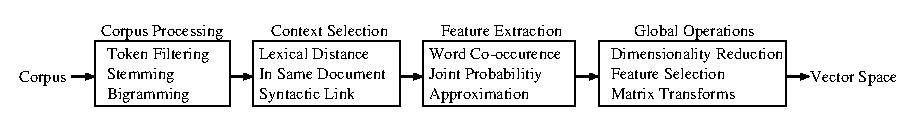
\includegraphics[width=1\textwidth]{figures/s-space-alg.eps}
  \caption{A high-level depiction of common algorithmic steps that convert a
    corpus into a word space}
  \label{fig:algorithm} 
\end{figure*}

Word space algorithms consist of the same core algorithmic steps: word features
are extracted from a corpus and the distribution of these features is used as a
basis for semantic similarity.  Figure \ref{fig:algorithm} illustrates the
shared algorithmic structure of all the approaches, which is divided into four
components: corpus processing, context selection, feature extraction and global
vector space operations.

Corpus processing normalizes the input to create a more uniform set of features
on which the algorithm can work.  Corpus processing techniques frequently
include stemming and filtering of stop words or low-frequency words.  For
web-gathered corpora, these steps also include removal of non linguistic tokens,
such as html markup, or restricting documents to a single language.

Context selection determines which tokens in a document may be considered for
features.  Common approaches use a lexical distance, syntactic relation, or
document co-occurrence to define the context.  The various decisions for
selecting the context accounts for many differences between otherwise similar
approaches.

Feature extraction determines the dimensions of the vector space by selecting
which tokens in the context will count as features.  Features are commonly word
co-occurrences, but more advanced models may perform a statistical analysis to
select only those features that best distinguish word meanings.  Other models
approximate the full set of features to enable better scalability.

Global vector space operations are applied to the entire space once the initial
word features have been computed.  Common operations include altering feature
weights and dimensionality reduction.  These operations are designed to improve
word similarity by changing the feature space itself.

\section{The S-Space Framework}

The S-Space framework is designed to be extensible, simple to use, and scalable.
We achieve these goals through the use of Java interfaces, reusable word space
related data structures, and support for multi-threading.  Each word space
algorithm is designed to run as a stand alone program and also to be used as a
library class.

\subsection{Reference Algorithms}

The package provides reference implementations for twelve word space algorithms,
which are listed in Table \ref{tab:algorithms}.  Each algorithm is implemented
in its own Java package, and all commonalities have been factored out into
reusable library classes.  The algorithms implement the same Java interface,
which provides a consistent abstraction of the four processing stages.

\begin{table}[tb]
  \small
  \begin{tabular}{l}
    \toprule
    \multicolumn{1}{c}{\bf Document-Based Models} \\
    LSA \cite{landauer97solution} \\
    ESA \cite{gabrilovich07computing} \\
    Vector Space Model \cite{salton75vector} \\

    \midrule
    \multicolumn{1}{c}{\bf Co-occurrence Models} \\
    HAL \cite{burgess97modeling} \\
    COALS \cite{rohde09improved} \\

    \midrule
    \multicolumn{1}{c}{\bf Approximation Models} \\
    Random Indexing \cite{sahlgren08permutations} \\
    Reflective Random Indexing \cite{cohen2009reflective} \\
    TRI \cite{jurgens09event} \\
    BEAGLE \cite{jones06high} \\
    Incremental Semantic Analysis \cite{baroni07isa} \\

    \midrule
    \multicolumn{1}{c}{\bf Word Sense Induction Models} \\
    Purandare and Pedersen \cite{purandare04word} \\
    HERMIT \cite{jurgens10improving} \\
    \bottomrule
  \end{tabular}
  \caption{Algorithms in the S-Space Package}
  \label{tab:algorithms}
\end{table}


We divide the algorithms into four categories based on their structural
similarity: document-based, co-occurrence, approximation, and Word Sense
Induction (WSI) models.  Document-based models divide a corpus into discrete
documents and construct the vector space from word frequencies in the documents.
The documents are defined independently of the words that appear in them.
Co-occurrence models build the vector space using the distribution of
co-occurring words in a context, which is typically defined as a region around a
word or paths rooted in a parse tree.  The third category of models approximate
co-occurrence data rather than model it explicitly in order to achieve better
scalability for larger data sets.  WSI models also use co-occurrence but also
attempt to discover distinct word senses while building the vector space.  For
example, these algorithms might represent ``earth'' with two vectors based on
its meanings ``planet'' and ``dirt.''

\subsection{Data Structures and Utilities}

The S-Space Package provides efficient implementations for matrices, vectors,
and specialized data structures such as multi-maps and tries.  Implementations
are modeled after the {\tt \footnotesize java.util} library and offer concurrent
implementations when multi-threading is required.  In addition, the libraries
provide support for converting between multiple matrix formats, enabling
interaction with external matrix-based programs.  The package also provides
support for parsing different corpora formats, such as XML or email threads.

\subsection{Global Operation Utilities}

Many algorithms incorporate dimensionality reduction to smooth their feature
data, e.g.\ \cite{landauer97solution,rohde09improved}, or to improve efficiency,
e.g.\ \cite{sahlgren08permutations,jones06high}.  The S-Space Package supports
two common techniques: the Singular Value Decomposition (SVD) and randomized
projections.  All matrix data structures are designed to seamlessly integrate
with six SVD implementations for maximum portability, including
SVDLIBJ\footnote{\texttt{\scriptsize
    http://bender.unibe.ch/svn/codemap/Archive/svdlibj/}} , a Java port of
SVDLIBC\footnote{\texttt{\scriptsize http://tedlab.mit.edu/\~dr/SVDLIBC/}}, a
scalable sparse SVD library.  The package also provides a comprehensive library
for randomized projections, which project high-dimensional feature data into a
lower dimensional space.  The library supports both integer-based projections
\cite{kanerva00random} and Gaussian-based \cite{jones06high}.

The package supports common matrix transformations that have been applied to
word spaces: point wise mutual information \cite{lin98automatic}, term
frequency-inverse document frequency \cite{salton88term},
and log entropy
\cite{landauer97solution}.

\subsection{Measurements}

The choice of similarity function for the vector space is the least standardized
across approaches.  Typically the function is empirically chosen based on a
performance benchmark and different functions have been shown to provide
application specific benefits \cite{weeds04characterising}.
To facilitate exploration of the similarity function parameter space, the
S-Space Package provides support for multiple similarity functions: cosine
similarity, Euclidean distance, KL divergence, Jaccard Index, Pearson
product-moment correlation, Spearman's rank correlation, and Lin Similarity
\cite{lin98automatic}

\subsection{Clustering}

Clustering serves as a tool for building and refining word spaces.  WSI
algorithms, e.g.\  \cite{purandare04word}, use clustering to discover the
different meanings of a word in a corpus. The S-Space Package provides bindings
for using the CLUTO clustering package\footnote{\texttt{\scriptsize
    \url{http://glaros.dtc.umn.edu/gkhome/views/cluto}}}.  In addition, the
package provides Java implementations of Hierarchical Agglomerative Clustering,
Spectral Clustering \cite{kannan04clusterings}, and the Gap Statistic
\cite{tibshirani00estimating}.

\section{Benchmarks}
\label{sec:benchmarks}

\begin{table*}[htb]
  \center
  \begin{threeparttable}
    \begin{tabular}{l l r ccc r ccc }
      \toprule
      & & &  \multicolumn{3}{c}{Word Choice} & &
      \multicolumn{3}{c}{Word Association} \\
      \cmidrule{4-6} \cmidrule{8-10}
      Algorithm & Corpus && TOEFL & ESL    & RDWP & & R-G    & WordSim353 & Deese \\
      \midrule
      \midrule
      BEAGLE    & TASA  &&  46.03  &  35.56  &  46.99  &&  0.431  &  0.342 & 0.235 \\
      COALS & TASA  &&  65.33  &  \textbf{60.42}  &  \textbf{93.02}  &&  0.572  &  0.478 & \textbf{0.388} \\
      HAL       & TASA  &&  44.00  &  20.83  &  50.00  &&  0.173  &  0.180 & 0.318 \\
      HAL       & Wiki  &&  50.00  &  31.11  &  43.44  &&  0.261  &  0.195 & 0.042 \\
      ISA       & TASA  &&  41.33  &  18.75  &  33.72  &&  0.245  &  0.150 & 0.286 \\
      LSA       & TASA  &&  56.00\tnote{a}  &  50.00  &  45.83  &&  0.652  &  0.519 & 0.349 \\
      LSA       & Wiki  &&  60.76  &  54.17  &  59.20  &&  \textbf{0.681}  &  \textbf{0.614} & 0.206 \\
      P\&P      & TASA  &&  34.67  &  20.83  &  31.39  &&  0.088  & -0.036 & 0.216 \\
      RI        & TASA  &&  42.67  &  27.08  &  34.88  &&  0.224  &  0.201 & 0.211 \\
      RI        & Wiki    &&  \textbf{68.35}  &  31.25  &  40.80  &&  0.226  &  0.315 & 0.090 \\
      RI $+$ Perm.\tnote{b}& TASA  &&  52.00  &  33.33  &  31.39  &&  0.137  &  0.260 & 0.268 \\
      RRI       & TASA  &&  36.00  &  22.92  &  34.88  &&  0.088  &  0.138 & 0.109 \\
      VSM       & TASA  &&  61.33  &  52.08  &  84.88  &&  0.496  &  0.396 & 0.200 \\
      \bottomrule
    \end{tabular}
    \begin{tablenotes}
    \item[a] {\footnotesize Landauer et al.\ \shortcite{landauer97solution}
      report a score of 64.4 for this test, while Rohde et
      al. \shortcite{rohde09improved} report a score of 53.4.}
    \item[b] {\footnotesize $+$ Perm indicates that permutations were used with
      Random Indexing, as described in \cite{sahlgren08permutations}}
    \end{tablenotes}
  \end{threeparttable}
  \caption{A comparison of the implemented algorithms on common evaluation
    benchmarks}
  \label{tab:evaluation}
\end{table*}

Word space benchmarks assess the semantic content of the space through analyzing
the geometric properties of the space itself.  Currently used benchmarks assess
the semantics by inspecting the representational similarity of word pairs.  Two
types of benchmarks are commonly used: word choice tests and association tests.
%
The S-Space Package supports six tests, and has an easily extensible model for
adding new tests.

\subsection{Word Choice}

Word choice tests provide a target word and a list of options, one of which has
the desired relation to the target.  Word space models solve these tests by
selecting the option whose representation is most similar.  Three word choice
benchmarks that measure synonymy are supported.

The first test is the widely-reported Test of English as a Foreign Language
(TOEFL) synonym test from \cite{landauer98introduction}, which consists of 80
multiple-choice questions with four options.  The second test comes from the
English as a Second Language (ESL) exam and consists of 50 question with four
choices \cite{turney01mining}.  The third consists of 200 questions from the
Canadian Reader's Digest Word Power (RDWP) \cite{jarmasz03rogets}, which unlike
the previous two tests, allows the target and options to be multi-word phrases.

\subsection{Word Association}

Word association tests measure the semantic relatedness of two words by
comparing word space similarity with human judgements.  Frequently, these tests
measure synonymy; however, other types of word relations such as antonymy
(``hot'' and ``cold'') or functional relatedness (``doctor'' and ``hospital'')
are also possible.  The S-Space Package supports three association tests.

The first test uses data gathered by Rubenstein and Goodneough
\shortcite{rubenstein65contextual}.  To measure word similarity, word similarity
scores of 51 human reviewers were gathered a set of 65 noun pairs, scored on a
scale of 0 to 4.  The ratings are then correlated with word space similarity
scores.

Finkelstein et al.\ \shortcite{finkelstein02placing} test for relatedness.  353
word pairs were rated by either 13 or 16 subjects on a 0 to 10 scale for how
related the words are.  This test is notably more challenging for word space
models because human ratings are not tied to a specific semantic relation.

The third benchmark considers the antonym association.  Deese
\shortcite{deese64associative} introduced 39 antonym pairs that Greffenstette
\shortcite{grefenstette92finding} used to assess whether a word space modeled
the antonymy relationship.  We quantify this relationship by measuring the
similarity rank of each word in an antonym pair, $w_1,w_2$, i.e.\  $w_2$ is the
$k^{th}$ most-similar word to $w_1$ in the vector space.  The antonym score is
calculated as $\frac{2}{rank_{w_1}(w_2) + rank_{w_2}(w_1)}$.  The score ranges
from $[0,1]$, where $1$ indicates that the most similar neighbors in the space are
antonyms.  We report the mean score for all 39 antonyms.

\section{Algorithm Analysis}

The content of a word space is fundamentally dependent upon the corpus used to
construct it.  Moreover, algorithms which use operations such as the SVD have a
limit to the corpora sizes they can process.  We therefore highlight the
differences in performance using two corpora.  TASA is a collection of 44,486
topical essays introduced in \cite{landauer97solution}.  The second corpus is
built from a Nov. 11, 2009 Wikipedia snapshot, and filtered to contain only
articles with more than 1000 words.  The resulting corpus consists of
387,082 documents and 917 million tokens.

Table \ref{tab:evaluation} reports the scores of reference algorithms on the six
benchmarks using cosine similarity.  The variation in scoring illustrates that
different algorithms are more effective at capturing certain semantic relations.
We note that scores are likely to change for different parameter configurations
of the same algorithm, e.g.\ token filtering or changing the number of
dimensions.

\begin{figure}[tb]
  \center
  \includegraphics[angle=270,width=.46\textwidth]{figures/timing.eps} 
  \caption{Processing time across different corpus sizes for a word space with
    the 100,000 most frequent words}
  \label{fig:sspace_timing} 
\end{figure}

\begin{figure}[tb]
  \center
  \includegraphics[angle=270,width=.46\textwidth]{figures/threading.eps} 
  \caption{Run time improvement as a factor of increasing the number of
    threads}
  \label{fig:sspace_threads} 
\end{figure}


As a second analysis, we report the efficiency of reference implementations by
varying the corpus size and number of threads.  Figure \ref{fig:sspace_timing}
reports the total amount of time each algorithm needs for processing
increasingly larger segments of a web-gathered corpus when using 8 threads. In
all cases, only the top 100,000 words were counted as features.  Figure
\ref{fig:sspace_threads} reports run time improvements due to multi-threading on
the TASA corpus.

Algorithm efficiency is determined by three factors: contention on global
statistics, contention on disk I/O, and memory limitations.  Multi-threading
benefits increase proportionally to the amount of work done per context.  Memory
limitations account for the largest efficiency constraint, especially as the
corpus size and number of features grow.  Several algorithms lack data points
for larger corpora and show a sharp increase in running time in Figure
\ref{fig:sspace_timing}, reflecting the point at which the models no longer fit
into 8GB of memory.

\section{Future Work and Conclusion}

We have described a framework for developing and evaluating word space
algorithms.  Many well known algorithms are already provided as part of the
framework as reference implementations for researches in distributional
semantics.  We have shown that the provided algorithms and libraries scale
appropriately.  Last, we motivate further research by illustrating the
significant performance differences of the algorithms on six benchmarks.

Future work will be focused on providing support for syntactic features,
including dependency parsing as described by \cite{pado07dependency}, reference
implementations of algorithms that use this information, more non-linear
dimensionality reduction techniques, and more advanced clustering algorithms.

\bibliographystyle{acl}
\bibliography{acl-sspace-paper}

\end{document}
